\section{Problem 4}
\textit{Alfa equal 55 degrees is claimed to be a good references – why? B) and why then measure in both 0, 90, 45 and -45 degrees and not 55 degrees?}

To make an evaluation of the environment it is needed to minimize the effect produced by the different polarizations in the received waves in such area. To reduce this effect it can be proved that for a half-length dipole, the mean effective gain (MEG) is the same independently of the cross polarization ratio $XPR$, when said dipole is inclined 55 degrees in its elevation angle.

When said dipole is inclined, it defines a plane (called antenna inclination plane in the bibliography). Subsequently, to evaluate the environment in which the antenna is located, this antenna inclination plane is then rotated in $\Phi$ (the azimuth angle) and the power measurements are performed.

In \figref{fig:dipole_inclination} it can be seen the angle $\alpha$ (which is set to 55 degrees in the experiment) and the angle $\Phi$ in which the antenna inclination angle is rotated. It can be mention that in the figure, the vector $L$ is in the antenna inclination plane.


\begin{figure}[!h]
  \centering
  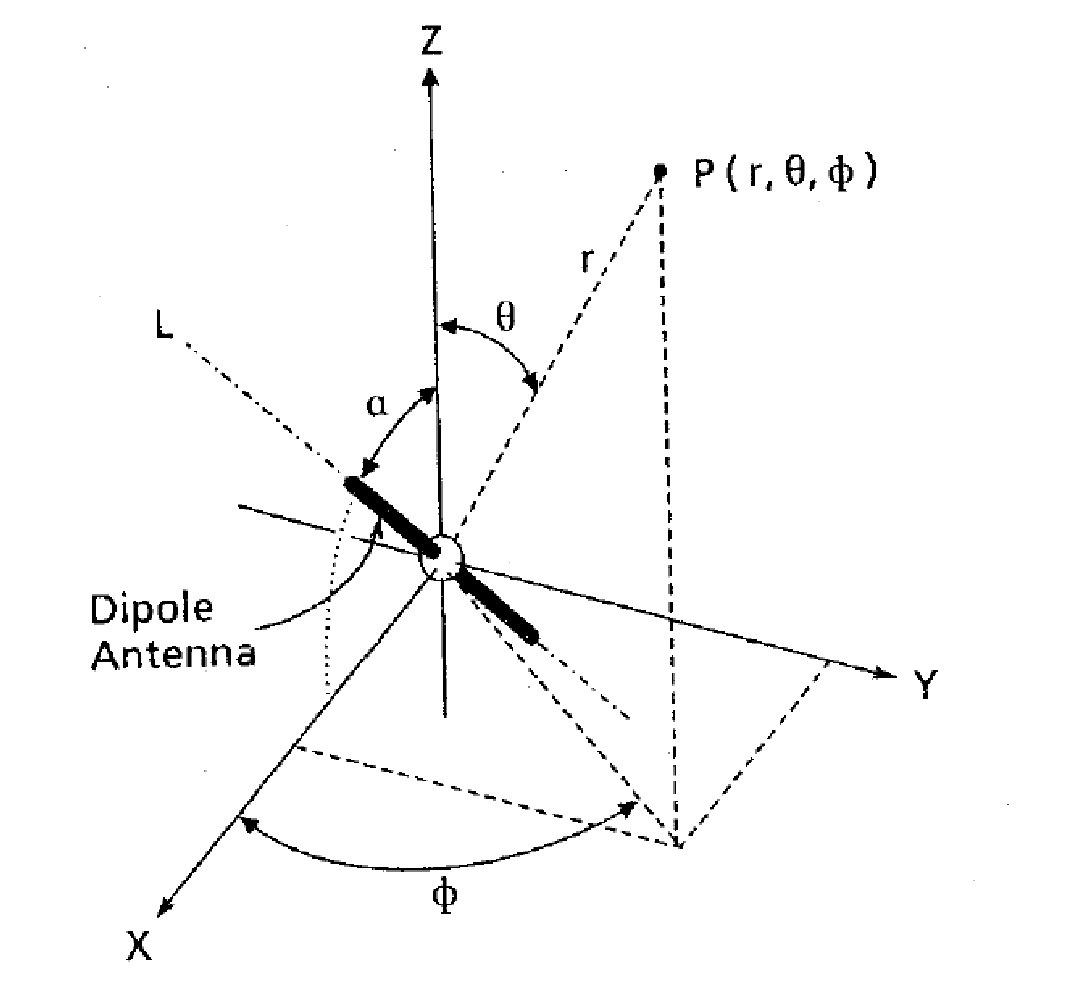
\includegraphics[width=10cm]{dipole_inclination.eps}
  \caption{Figure showing the angles involved in the dipole inclination and rotation (WRITE SOURCE)}
  \label{fig:dipole_inclination}
\end{figure}

As it is commented before, with this inclination the Prec is half of Pv+Ph independently from the XPR. Then, is a good reference to evaluate the MEG of the antenna without knowing the XPR of the signal transmitted.
The 0, 90, 45 and -45 degrees correspond to the different orientation of the inclination plane of the antenna. As it is shown in \figref{fig:street_nr} and \figref{fig:street_r}, it is important the scenario where the route is taking place, given the fact that high buildings cause a ‘cannon’ effect in which the signal is mainly received in the direction of the street.

\begin{figure}[!h]
  \centering
  \includegraphics[width=10cm]{street_nr.eps}
  \caption{Representation of the scenario when the inclination plane is not rotated($\Phi=0$)}
  \label{fig:street_nr}
\end{figure}

\begin{figure}[!h]
  \centering
  \includegraphics[width=10cm]{street_r.eps}
  \caption{Representation of the scenario when the inclination plane is rotated($\Phi\neq0$)}
  \label{fig:street_r}
\end{figure}
